\section{$C^1$ Finite Element Discretisation}
\label{sec:fem}

\subsection{Bogner--Fox--Schmit Bicubic Hermite Element}
The displacement-based Mindlin Form-II weak form requires second derivatives. Standard $C^0$ Lagrange interpolation is therefore insufficient for an $H^2(\Omega)$-conforming formulation. We use the Bogner--Fox--Schmit (BFS) bicubic element, which is $C^1$-conforming on structured rectangular meshes \cite{bfs1965}.

For a rectangular element of dimensions $2a \times 2b$, we interpolate $u_1(x, y)$ and $u_2(x, y)$ independently, using tensor products of one-dimensional cubic Hermite polynomials:
\begin{equation}
u_i(x, y) = \sum_{a=1}^4 \sum_{p=1}^4 N_{a,p}(x, y) d_{i, a, p}^e, \quad i \in \{1, 2\},
\label{eq:bfs_interpolation}
\end{equation}
where $a \in \{1, 2, 3, 4\}$ indexes the four element vertices, and $p \in \{1, 2, 3, 4\}$ denotes the four nodal degrees of freedom per displacement component:
\begin{equation}
\setlength{\arraycolsep}{3.5pt}
\bm{d}_{i, a}^e = \begin{bmatrix} u_i & \frac{\partial u_i}{\partial x} & \frac{\partial u_i}{\partial y} & \frac{\partial^2 u_i}{\partial x \partial y} \end{bmatrix}^\mathsf{T}_{\text{at node } a}.
\label{eq:nodal_dof_vector}
\end{equation}
Each vertex has four degrees of freedom for each displacement component, giving 32 per element. Figure~\ref{fig:bfs_dof} shows their Bloch-phase mapping. All reported band structures and design maps use a uniform mesh of $n \times n = 16 \times 16$ BFS elements per unit cell. This gives $h=L/n=0.0625$ and $8n^2=2048$ independent degrees of freedom per cell. Here $8n^2$ is the count after Bloch reduction. The Case-C mesh data instead use the assembled count $8(N+1)^2$ before reduction.

\begin{figure*}[htbp]
\centering
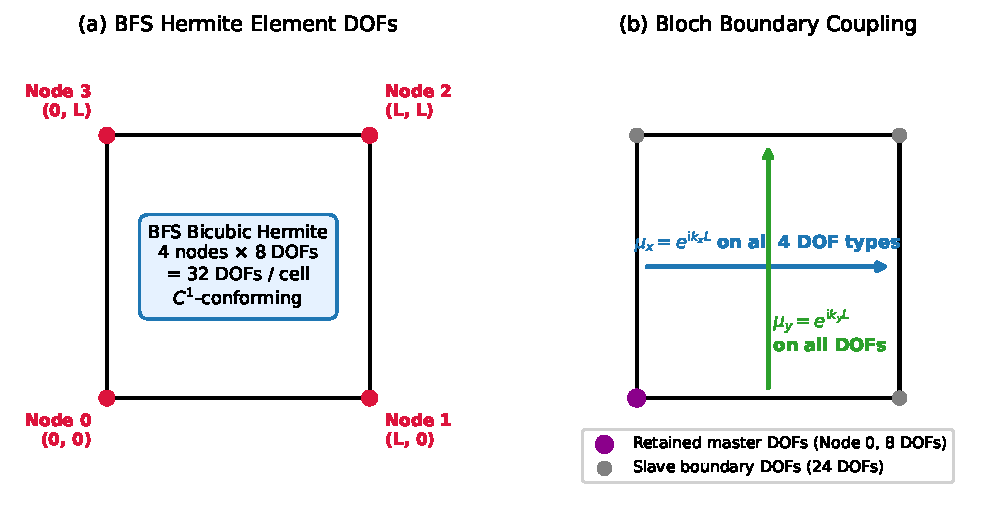
\includegraphics[width=\textwidth]{figures/fig03_bfs_dof_bloch.pdf}
\caption{BFS finite element. (a) Nodal degrees of freedom. (b) Bloch coupling of displacement and derivative degrees of freedom at paired boundaries.}
\label{fig:bfs_dof}
\end{figure*}

\subsection{Element matrices}
The strain tensor $\bm\varepsilon$ and strain-gradient tensor $\bm\eta$ within element $e$ are related to the element nodal displacement vector $\bm{d}^e \in \mathbb{R}^{32}$ through the kinematic strain--displacement matrices $\bmB^c$ and $\bmB^g_k$:
\begin{equation}
\begin{split}
\bm\varepsilon &= \bmB^c \bm{d}^e,\\
\bm\eta_k &\equiv \frac{\partial \bm\varepsilon}{\partial x_k} = \bmB^g_k \bm{d}^e, \quad k \in \{1, 2\}.
\end{split}
\label{eq:strain_matrices}
\end{equation}
The element stiffness matrix $\bmK^e$ has a classical part and a gradient part:
\begin{equation}
\bmK^e = \bmK^c + \bmK^g(\theta, \mathrm{AR}),
\label{eq:Ke_total}
\end{equation}
The classical stiffness matrix is:
\begin{equation}
\bmK^c = \int_{\Omega_e} (\bmB^c)^\mathsf{T} \bmC \bmB^c \,\dif\Omega,
\label{eq:Kc_int}
\end{equation}
The anisotropic gradient stiffness matrix is:
\begin{equation}
\bmK^g(\theta, \mathrm{AR}) = \frac{1}{10} \sum_{k=1}^2 \sum_{l=1}^2 L_{kl}(\theta) \int_{\Omega_e} (\bmB^g_k)^\mathsf{T} \bmC \bmB^g_l \,\dif\Omega.
\label{eq:Kg_int}
\end{equation}
In a homogeneous element, the stiffness and mass integrands have degree at most six in each coordinate. Four Gauss--Legendre points integrate polynomials up to degree seven exactly. A $4\times4$ rule is therefore enough. This avoids quadrature error for homogeneous elements. The unconstrained stiffness still has its expected rigid-body null modes. For elements intersected by the inclusion, we use sub-cell Gauss sampling with an $O(h)$ geometric approximation.

\subsubsection{Mass and micro-inertia matrices}
The kinetic energy gives the classical and micro-inertia mass contributions:
\begin{equation}
\bmM^e = \bmM_0 + \ell_{\mathrm{i}}^2 \bmM^g,
\label{eq:Me_total}
\end{equation}
with:
\begin{equation}
\begin{split}
\bmM_0 &= \rho \int_{\Omega_e} \bm{N}^\mathsf{T} \bm{N} \,\dif\Omega, \\
\bmM^g &= \rho \sum_{k=1}^2 \int_{\Omega_e} \left(\frac{\partial \bm{N}}{\partial x_k}\right)^\mathsf{T} \left(\frac{\partial \bm{N}}{\partial x_k}\right) \,\dif\Omega.
\end{split}
\label{eq:Mg_int}
\end{equation}
Both $\bmM_0$ and $\bmM^g$ are symmetric and positive semi-definite. Their sum $\bmM^e$ is strictly positive definite for any $\rho > 0$.

\subsection{Bloch reduction and eigenproblem}
To impose the Bloch conditions on $\partial\Omega_{\mathrm{cell}}$, we split the global degrees of freedom $\bm{d}$ into interior ($I$), master-boundary ($M$) and slave-boundary ($S$) sets:
\begin{equation}
\bm{d} = \begin{bmatrix} \bm{d}_I \\ \bm{d}_M \\ \bm{d}_S \end{bmatrix}.
\label{eq:d_partition}
\end{equation}
The Bloch transformation links the slave DOFs on the top and right boundaries to the master DOFs on the bottom and left boundaries:
\begin{equation}
\bm{d}_S = \bmT_{SM}(\bmk) \bm{d}_M,
\label{eq:slave_master_rel}
\end{equation}
Here $\bmT_{SM}(\bmk)$ is a diagonal complex phase matrix. Its entries are $e^{\iu k_x L}$, $e^{\iu k_y L}$ or $e^{\iu (k_x + k_y)L}$ for each periodic node pair. Displacement and derivative degrees of freedom share the same phase multiplier.

In the continuous weak form, the natural boundary work cancels between opposite cell faces. The effective traction $p_i^{\mathrm{dyn}}$ carries the Bloch phase and changes sign with the outward normal. Its test trace carries the conjugate phase. The double traction $R_i=n_jn_k\tau_{ijk}$ also carries the Bloch phase, but it keeps its sign when the normal reverses. Its work-conjugate normal derivative changes sign. Together, these signs and phases cancel both face integrals. Line and corner terms pair under the same translations. At the corner, the product phase $e^{\iu(k_x+k_y)L}$ appears. No separate free-boundary condition is imposed on a Bloch-paired face.

We collect these relations in the master--slave transformation matrix $\bmT(\bmk)$:
\begin{equation}
\begin{split}
\bm{d} &= \bmT(\bmk) \bar{\bm{d}}, \quad \bar{\bm{d}} = \begin{bmatrix} \bm{d}_I \\ \bm{d}_M \end{bmatrix}, \\
\bmT(\bmk) &= \begin{bmatrix} \mathbf{I}_{II} & \mathbf{0} \\ \mathbf{0} & \mathbf{I}_{MM} \\ \mathbf{0} & \bmT_{SM}(\bmk) \end{bmatrix},
\end{split}
\label{eq:T_bloch}
\end{equation}
Galerkin projection gives the reduced stiffness and mass matrices:
\begin{equation}
\begin{split}
\bar{\bmK}(\bmk) &= \bmT(\bmk)^\mathsf{H} \bmK \bmT(\bmk), \\
\bar{\bmM}(\bmk) &= \bmT(\bmk)^\mathsf{H} \bmM \bmT(\bmk).
\end{split}
\label{eq:reduced_KM}
\end{equation}

\subsubsection{Reduced Hermitian eigenproblem}
We obtain the dispersion curves $\barw_n(\bmk)$ from the reduced generalised eigenvalue problem:
\begin{equation}
\left[ \bar{\bmK}(\bmk) - \omega^2 \bar{\bmM}(\bmk) \right] \bar{\bm{d}} = \bm{0}.
\label{eq:eigenproblem}
\end{equation}
Each entry of the diagonal phase subblock $\bmT_{SM}(\bmk)$ has unit modulus, so this subblock is unitary. The full matrix $\bmT(\bmk)$ is rectangular with full column rank. Unlike the phase subblock, it is not unitary. For positive elastic and inertial parameters, the full-cell matrices satisfy $\bmK\succeq 0$ and $\bmM\succ 0$. The reduced operators are therefore Hermitian:
\begin{equation}
\begin{split}
\bar{\bmK}(\bmk)^\mathsf{H} &= \bar{\bmK}(\bmk) \succeq 0, \\
\bar{\bmM}(\bmk)^\mathsf{H} &= \bar{\bmM}(\bmk) \succ 0,
\end{split}
\label{eq:hermiticity}
\end{equation}
The generalised eigenvalues $\omega_n^2$ are therefore real and non-negative. Shifting $\bmk$ by a reciprocal-lattice vector $\bm{G}$ leaves every Bloch phase unchanged, so the reduced stiffness and mass matrices satisfy $\bar{\bmK}(\bmk + \bm{G}) = \bar{\bmK}(\bmk)$ and $\bar{\bmM}(\bmk + \bm{G}) = \bar{\bmM}(\bmk)$. The spectrum is periodic across reciprocal space.

\subsubsection{Branch tracking}
Modes of different spatial symmetry can cross along high-symmetry paths. To follow a mode between adjacent wave vectors, we use the Modal Assurance Criterion (MAC) at $\bmk_1$ and $\bmk_2$. Let $\bm{d}_m(\bmk)=\bmT(\bmk)\bar{\bm{d}}_m(\bmk)$ be the full-cell eigenvector. Let $\bmM$ be the common assembled full-cell mass matrix, which includes gradient micro-inertia. The cross-wavevector MAC is
\begin{equation}
{\small
\mathrm{MAC}_{mn}(\bmk_1,\bmk_2) = \frac{\left| \bm{d}_m(\bmk_1)^\mathsf{H} \bmM \bm{d}_n(\bmk_2) \right|^2}{\left( \bm{d}_m(\bmk_1)^\mathsf{H} \bmM \bm{d}_m(\bmk_1) \right) \left( \bm{d}_n(\bmk_2)^\mathsf{H} \bmM \bm{d}_n(\bmk_2) \right)}
}
\label{eq:mac_def}
\end{equation}
The MAC uses the common full-cell mass matrix because the reduced mass matrix depends on $\bmk$. A direct comparison of reduced eigenvectors would therefore be inconsistent. If the off-diagonal MAC indicates a branch exchange, we halve the continuation step. We compute band gaps from the frequency-ordered eigenvalues $\barw_1(\bmk) \le \barw_2(\bmk) \le \dots \le \barw_N(\bmk)$, independently of the mode labels assigned during tracking.
